\documentclass{article}
\usepackage{style}

\author{Jorge Gómez Reus}
\date{}
\begin{document}
\maketitle
\tableofcontents
\section{Sistema Lineal}
Es aquel que posee le propiedad de superposición: Si una entrada consiste en la suma ponderada de varias señales, entonces la salida es simplemente la suma ponderada (superposición) de las respuestas del sistema a cada una de las señales.\\
Propiedades: 
\begin{enumerate}
	\item Aditividad:\\
	\begin{figure}[h!]
		\centering
		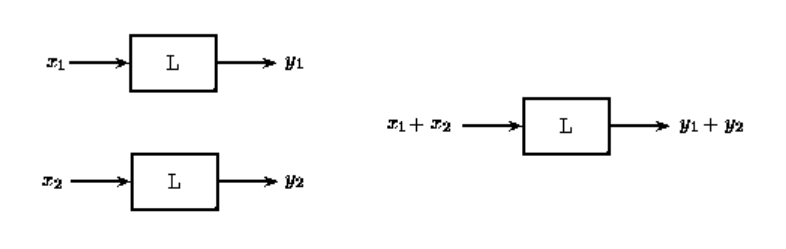
\includegraphics[scale=.8]{img/aditivity}
	\end{figure} 
	\item Escalamiento u Homogeniedad
	\begin{figure}[h!]
		\centering
		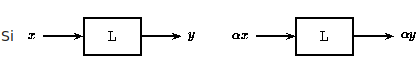
\includegraphics[scale=.8]{img/proportionality}
	\end{figure} 
\end{enumerate}
Las dos propiedades que definen un sistema lineal combinadas se conocen como superposición:
\begin{itemize}
	\item Tiempo continuo: $ax_1(t) + bx_2(t) \rightarrow ay_1(t) + by_2(t)$\\
	$$y[n] = \sum_{k}=a_{k}x_{k}[n] = a_1x_1[n] + a_2x_2[n] + a_3x_3[n] + \ldots$$
	\item Tiempo Discreto: $ax_1[n] + bx_2[n] \rightarrow ay_1[n] + by_2[n]$\\
	$$y[n] = \sum_{k}=a_{k}y_{k}[n] = a_1y_1[n] + a_2y_2[n] + a_3y_3[n] + \ldots$$
\end{itemize}
Una consecuencia directa de la propiedad de superposición es que para sistemas lineales, una entrada que sea cero en todo tiempo da una salida de en todo tiempo.
\section{Ejemplos}
\end{document}
